%------------------------ Packages ------------------------
\documentclass[12pt,a4paper]{article}
\usepackage[latin1]{inputenc}
\usepackage[T1]{fontenc}
\usepackage[pdftex]{graphicx}
\usepackage{float}
\usepackage{amsmath}
\usepackage{amssymb}
\usepackage[FIGTOPCAP]{subfigure}
\usepackage{color}
\usepackage[hidelinks]{hyperref}

\newcommand{\version}{\IfFileExists{../../version.txt}
{\input{../../version.txt}}
{\input{../../../version.txt}}
}

\newcommand{\command}[1]{%
\indent \fcolorbox{black}{white}{%
   \begin{minipage}{\dimexpr\textwidth-\parindent\relax}%
      #1
   \end{minipage}%
}
}

\newsavebox{\FVerbBox}
\newenvironment{sample}
{\par \vspace{0.2cm} \begin{lrbox}{\FVerbBox}
\begin{minipage}{\dimexpr\textwidth-\parindent\relax}}
{\end{minipage}
\end{lrbox}
\fcolorbox{black}{lightgray}{\usebox{\FVerbBox}}
\vspace{0.2cm}}

\newenvironment{sampletitle}
{\vspace{0.2cm} \noindent\textbf{Example} :
\begin{sample}}
{\end{sample}}

\newcommand{\samplecomment}[1]{%

\textit{#1}
}

\newcommand{\seealso}[1]{\vspace{0.2cm} \noindent\textbf{See also} :\par #1}

% tikz
\usetikzlibrary{calc}
\usetikzlibrary{arrows}
\usetikzlibrary{shadows}

\tikzset{block/.style={draw, text centered, fill=gray!10,drop shadow}}
\tikzset{connect/.style={draw, line width=1 pt}}

\begin{document}

\begin{center}
\textbf{\huge  \underline{Erosion operator}}
\end{center}
\vspace{0.5cm}

The erosion operator is a morphological operation used to amplify the surface of the dark areas in the image. In a greyscale image, all the dark areas are amplified, while on binary images black spots are enlarged.
At each point in the image, the minimal value of the selected neighbours is the new value of the central point.\\


\begin{figure}[h!]
\centering
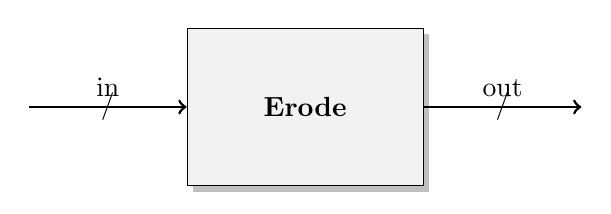
\begin{tikzpicture}
\node[block,rectangle,minimum height=2cm,minimum width=3cm] (bloc) {\textbf{Erode}};

\path[connect,<-] ([yshift=0.0cm]bloc.west) -- node{/} node[above]{in} ++(-2cm,0);

\path[connect,->] ([yshift=0.0cm]bloc.east) -- node{/} node[above]{out} ++(2cm,0);
 ([xshift=0.5cm,yshift=-0.6cm]bloc.north);

\end{tikzpicture}
\end{figure}

\vspace{0.5cm}

\begin{figure}[!h]
\centering
\subfigure[Initial greyscale image]{
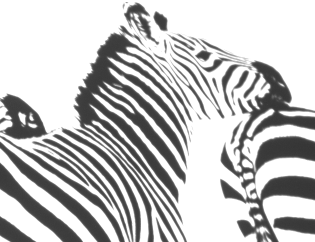
\includegraphics[width=5cm]{greyscale.png}}
\hspace{2cm}
\subfigure[Erode image]{
\includegraphics[width=5cm]{erode1.png}}
\vspace{2cm}
\subfigure[Initial binary image]{

\includegraphics[width=5cm]{binary.png}}
\hspace{2cm}
\subfigure[Eroded binary image]{
\includegraphics[width=5cm]{erode2.png}}
\end{figure}

\section*{Properties}
\properties{
enable           & bool & Enable the processing \\ 
erosion\_ matrix & matrix & Structural element used to compare each point to its neighbours\\
}

\vspace{0.5cm}

\section*{Constants}

\constants{
LINE\_WIDTH\_MAX & Maximum line size of the image : 1280 pixels  \\ 
CLK\_PROC\_FREQ & Frequency clock of the process \\
IN\_SIZE & Size of the input flow : 1 byte (greyscale image) or 1 bit (binary image)\\
OUT\_SIZE & Size of the output flow : 1 byte (greyscale image) or 1 bit (binary image)\\
}



\section*{Equivalence}
\subsection*{Matlab}

\lstset{language=Matlab}
\begin{lstlisting}
I; % image matrix
SE = [0 1 0 ; 1 1 1 ; 0 1 0]; % Structural element 3x3
I_dilated = imerode(I,SE); % erosion operation on I with SE as a structuring element object.
% This functions takes a grayscale or a binary image

\end{lstlisting}

\url{https://fr.mathworks.com/help/images/ref/imerode.html}


\subsection*{OpenCV}

\lstset{language=C++}
\begin{lstlisting}
void erode(InputArray src, OutputArray dst, 
	InputArray kernel, Point anchor=Point(-1,-1), 
	int iterations=1, int borderType=BORDER_CONSTANT, 
	const Scalar& borderValue=morphologyDefaultBorderValue() 
	)

/*Parameters:	
    src – input image; the number of channels can be arbitrary, but the depth should be one of CV_8U, CV_16U, CV_16S, CV_32F` or ``CV_64F.
    dst – output image of the same size and type as src.
    element – structuring element used for erosion; if element=Mat() , a 3 x 3 rectangular structuring element is used.
    anchor – position of the anchor within the element; default value (-1, -1) means that the anchor is at the element center.
    iterations – number of times erosion is applied.
    borderType – pixel extrapolation method (see borderInterpolate() for details).
    borderValue – border value in case of a constant border (see createMorphologyFilter() for details).

*/
\end{lstlisting}

\url{http://docs.opencv.org/2.4/modules/imgproc/doc/filtering.html#erode}

\section*{Mathematical formalism}

The operator uses a $3x3$ binary kernel called "Structuring element" which is giving the neighbours to evaluate around each point of the image. \\

The generalization of erosion to gray-level images is that the gray-level value at any point is replaced by the $minimum$ intensity value covered by the flat structuring element. That is, pointwise erosion of the image $I$ by a flat structuring element $SE$ is defined as:\\


\centering
$\displaystyle I \oplus SE (\bf x )$ 	$\textstyle =$ 	$\displaystyle min \{I({\bf z}): {\bf z} \epsilon S_x \},$

\vspace{0.5cm}



\end{document}